%% GENERATED from paper_f_template.tex by scripts/build_paper_f.py. Do not edit.
%% Paper F: do rankings of explanation methods hold across tabular datasets?
%% Target: Journal of Computer Sciences Institute (JCSI). Rules: VENUE_JCSI.md.
%%
%% THIS IS THE SOURCE. paper_f.tex is GENERATED from it by scripts/build_paper_f.py, which
%% replaces \input{generated/...} fragments and \pending{alias:key} placeholders
%% with values read from result files. Edit this file, never paper_f.tex.
%%
%% The journal takes Word in its own template: A4, two columns of 8 cm, 1 cm between,
%% margins 2.5 cm (top, bottom) and 2 cm (left, right), Times New Roman 10 pt, single
%% spacing, 4 to 8 pages. This source is set to the same page so that the PDF predicts
%% the length. The submitted file is made in the journal's Word template.
%%
%% Review is double-blind. The default build omits author identity; the full build is
%% made by defining \fullversion before this file.
%%
%% DRAFT of 2026-10-05: introduction and methods follow ANALYSIS_PLAN.md (version 2).
%% 2026-10-11: the Results section is a skeleton wired to the analysis files, written
%% before the analysis was run. No number of the results, discussion or conclusions is
%% typed by hand: each is a placeholder or a visible "[pending]" mark.
%% 2026-10-11, after the analysis (results b7b8d576b): abstract, reading of Table 3,
%% discussion, sources of error and conclusions written from RESULTS_REPORT.md. Numbers
%% are still placeholders. No pending mark is left.
\documentclass[10pt,a4paper,twocolumn]{article}
\usepackage[top=25mm,bottom=25mm,left=20mm,right=20mm,columnsep=10mm]{geometry}
\usepackage{fontspec}
\setmainfont{texgyretermes}[Extension=.otf, UprightFont=*-regular, BoldFont=*-bold,
  ItalicFont=*-italic, BoldItalicFont=*-bolditalic]
\usepackage{amsmath}
\usepackage{amssymb}
\usepackage{graphicx}
\usepackage{booktabs}
\usepackage{array}
\usepackage{xcolor}
\usepackage[hidelinks]{hyperref}
\usepackage[numbers,sort&compress]{natbib}
\setlength{\emergencystretch}{3em}
\setlength{\bibsep}{2pt}
%% Figure 1 takes about 70% of a page; with the default limit it floats past the references.
\renewcommand{\dbltopfraction}{0.9}
\renewcommand{\textfraction}{0.1}
\providecommand{\fullurl}[1]{\url{#1}}  % used by entries taken from the Paper E list
\newcommand{\pending}[1]{\textcolor{red}{[pending: #1]}}
%% Code and data archive (full version only): Zenodo version 0.13.0, from GitHub release
%% paper-f-jcsi-2026-10-11 (2026-10-11). A change to code or results needs a new version.
\newcommand{\paperfarchive}{\url{https://doi.org/10.5281/zenodo.23307705}}

\newif\iffull
\ifdefined\fullversion \fulltrue \else \fullfalse \fi

\begin{document}

\twocolumn[
\begin{flushleft}
%% Title chosen by the author on 2026-10-05; not changed without the author's approval.
{\Large\bfseries How Dataset-Dependent Are Tabular Explainability Benchmarks?\par}
\medskip
\iffull
Jonathan Herrera-V\'asquez\textsuperscript{*}\par
\smallskip
{\small Department of Computer Science, Universidad Americana de Europa (UNADE),
Canc\'un, Quintana Roo, Mexico\par}
\else
\textit{Author information omitted for double-blind review.}\par
\fi
\medskip
\textbf{Abstract}\par
\smallskip
Explanation methods are usually compared on one dataset, and the resulting order is read
as a property of the methods. We test this for LIME, SHAP, Anchors and DiCE on four
classifiers and 16 public tabular datasets chosen by a fixed rule,
ranking the methods on faithfulness, stability, sparsity and cost. The mean rank
correlation between datasets is 0.67,
0.88, 0.79 and
0.87 for the four measures, above chance in all
($p$~$<$0.001); its 95\% interval lies above 0.5 except for faithfulness.
Much of this agreement follows from the output format and the settings of the methods,
not from the data. Of 24 pairwise orders found on the Adult
dataset, 12 hold on all 15 other datasets; the
order of Anchors and DiCE is the one that changes.

\medskip
\textit{Keywords}: explainable artificial intelligence; LIME; SHAP; benchmark;
external validity; tabular data
\medskip

\iffull
{\small \textsuperscript{*}Corresponding author. \textit{Email address}:
jonnabio@gmail.com (J. Herrera-V\'asquez). ORCID:
\url{https://orcid.org/0000-0002-7149-6635}\par}
\medskip
\fi
\hrule
\bigskip
\end{flushleft}
]

\section{Introduction}

A model that decides on credit or medical risk is often an ensemble of trees or a neural
network, too complex to be read directly~\cite{cerneviciene2024finance}. Those who decide
with such a model and those affected by its decisions need to know which inputs drove a
prediction, and they do not need the same explanation~\cite{kim2024stakeholder}. Post-hoc
explanation methods answer in three forms: LIME~\cite{ribeiro2016why} and
SHAP~\cite{lundberg2017unified} assign a weight to every feature, Anchors returns a rule
that keeps the prediction with high probability~\cite{ribeiro2018anchors}, and DiCE
returns counterfactual instances that change it~\cite{mothilal2020dice}. The methods
often disagree on the same prediction, and practitioners resolve the disagreement with
ad hoc heuristics~\cite{krishna2022disagreement}. Comparative studies, which score the
methods on properties such as faithfulness, stability, sparsity and cost, are therefore
the usual guide to a choice. Surveys list the evaluation of explanations among the open
problems of the field~\cite{longo2024manifesto,mersha2024survey}, also for tabular
data~\cite{obrienquinn2024tabular,santana2026tabular}.

The product of a comparative study is an order: on a given measure, one method is better
than another. A reader who adopts the method ranked first applies it to other data, and
so relies on an assumption the study seldom tests: that the order is a property of the
methods and not of the dataset on which they were compared. A large benchmark makes a
related criticism of current studies, which examine few methods and metrics, ignore the
model architecture and the nature of the input data, and yield unreliable
rankings~\cite{klein2024maze}. If the order changes from one dataset to the next, a
result obtained on a single benchmark says little about the choice a practitioner faces.

\subsection{Related work}

There is no single accepted measure of the quality of an explanation. A study of the
evaluation of local post-hoc methods on tabular data derives 20 criteria with guidelines
for each~\cite{velmurugan2025guidelines}; an examination of the many proposed metrics
finds duplication and calls for standard frameworks~\cite{pawlicki2024metrics}; and new
measures, benchmarks and metric studies continue to
appear~\cite{bello2025strength,sithakoul2024beexai,pereira2026local}. Where a ground
truth for the explanation can be built, methods differ clearly in
fidelity~\cite{mironicolau2024fidelity}.

The methods compared here have documented weaknesses: SHAP and LIME depend on the model
and on collinear features~\cite{salih2024perspective} and can credit features that a
model with known rules does not use~\cite{hooshyar2024problems}, Shapley values are
criticised as a basis for explanations~\cite{huang2024failings}, and different methods
explain the same prediction
differently~\cite{parashar2026agreement,gao2026uncertainty}. Rule-based and
counterfactual explanations remain active lines of
work~\cite{tekin2026fuzzy,redelmeier2024mcce}. Applied studies compare the methods on
one task: three methods on five datasets of different types in this
journal~\cite{kuszewska2026comparative}, four importance measures on one medical
dataset~\cite{biesaga2026comparison}, and LIME and SHAP on the prediction of software
issues~\cite{schulte2024studying}.

Whether an order found on one dataset holds on another has been examined for images: for
attribution maps, metric results on one dataset did not necessarily hold on
others~\cite{gevaert2024evaluating}. A recent benchmark of tabular classifiers
curates a representative collection of datasets~\cite{erickson2025tabarena}, and
tabular data are heterogeneous in feature types, cardinality and
sparsity~\cite{somvanshi2026survey}. Comparisons of explanation methods on tabular data
seldom use many datasets. The census income data known as Adult is a frequent
single benchmark, and a framework for measuring explanation quality was itself first
validated on it~\cite{herrera2026framework}.

\subsection{Purpose and hypothesis}

The purpose of this work is to measure how far the order of four explanation methods,
obtained on one tabular dataset, holds on other tabular datasets. The object of the
research is therefore the transfer of a comparative conclusion and not the quality of
any one method. The research covers binary classification on tabular data, four
classifiers of different families and four measures on which the four methods can all be
ranked.

The research hypothesis is: \textit{on each measure, the order of the four explanation
methods agrees across tabular datasets more than chance.} The hypothesis, the measures,
the rule for choosing the datasets and the decision rule were fixed in a plan committed
to a public repository before any explanation was computed.

\section{Materials and methods}

\subsection{Datasets}

The datasets were chosen by a rule and not by hand, so that the choice could not favour
one outcome. A dataset is included if it is public and usable without registration; is
tabular with a binary target; has at least 1,000 rows and between 5 and 100 features; and
if at least three of the four classifiers reach a cross-validated area under the ROC
curve between 0.65 and 0.98 on it, which removes datasets that are noise or trivially
separable. Candidates were taken from OpenML~\cite{vanschoren2014openml} in an order
fixed beforehand, in six strata defined by the type of the features (numeric, mixed,
categorical) and the number of rows (below or from 10,000).
When fewer than sixteen of the listed candidates passed, the list was extended with the
binary tasks of the OpenML-CC18 suite in the order of their identifier. Of
77 candidates listed, 16 are in the
study (Table~\ref{tab:datasets}). The minority class is the positive class.

\begin{table*}[t]
\centering
\caption{Datasets of the study. Features are counted before encoding.}
\label{tab:datasets}
\small
\begin{tabular}{llrrrrl}
\toprule
Dataset & OpenML id & Rows & Features & Numeric (\%) & Minority class (\%) & Stratum \\
\midrule
phoneme & 1489 & 5,404 & 5 & 100 & 29.3 & numeric, under 10,000 rows \\
qsar-biodeg & 1494 & 1,055 & 41 & 100 & 33.7 & numeric, under 10,000 rows \\
ozone-level-8hr & 1487 & 2,534 & 72 & 100 & 6.3 & numeric, under 10,000 rows \\
MagicTelescope & 1120 & 19,020 & 10 & 100 & 35.2 & numeric, from 10,000 rows \\
electricity & 151 & 45,312 & 8 & 88 & 42.4 & mixed, from 10,000 rows \\
default-of-credit-card-clients & 42477 & 30,000 & 23 & 100 & 22.1 & numeric, from 10,000 rows \\
credit-g & 31 & 1,000 & 20 & 35 & 30.0 & mixed, under 10,000 rows \\
churn & 40701 & 5,000 & 20 & 80 & 14.1 & mixed, under 10,000 rows \\
compas-two-years & 42192 & 5,278 & 13 & 54 & 47.0 & mixed, under 10,000 rows \\
adult & 1590 & 48,842 & 14 & 43 & 23.9 & mixed, from 10,000 rows \\
bank-marketing & 1461 & 45,211 & 16 & 44 & 11.7 & mixed, from 10,000 rows \\
Amazon\_employee\_access & 4135 & 32,769 & 9 & 0 & 5.8 & categorical, from 10,000 rows \\
pc4 & 1049 & 1,458 & 37 & 100 & 12.2 & numeric, under 10,000 rows \\
pc3 & 1050 & 1,563 & 37 & 100 & 10.2 & numeric, under 10,000 rows \\
jm1 & 1053 & 10,885 & 21 & 100 & 19.4 & numeric, from 10,000 rows \\
kc1 & 1067 & 2,109 & 21 & 100 & 15.5 & numeric, under 10,000 rows \\
\bottomrule
\end{tabular}
\end{table*}


Numeric features are standardised and missing values replaced by the median; categorical
features are one-hot encoded, with categories beyond the 20 most frequent of a feature
grouped into one level; the encoded datasets have 5
to 180 features. Each dataset is split into 80\% for
training and 20\% for testing, stratified by class.

\subsection{Classifiers and explanation methods}

Four classifiers are trained on every dataset with one configuration for all: logistic
regression, a random forest of 100 trees,
XGBoost with 100 trees of depth 4, and a multilayer perceptron
with one hidden layer of 100 units.

The four explanation methods are also used with one configuration for all datasets and
no tuning: LIME with 1,000 samples, 10 features and a kernel width of 3; SHAP with 50
background rows, in its exact tree variant for the two tree models and its kernel variant
for the other two; Anchors with a precision threshold of 0.95; and DiCE with random
search for one counterfactual, the encoded columns being treated as continuous.
Explanations are computed on the encoded features.

\subsection{Research scenario}

The design is a full factorial. Each of the 16 datasets is combined
with the four classifiers and the four methods, and every combination is repeated with
five seeds: 42, 123, 456, 789 and 101112. The values carry no meaning;
they were written in the configuration file before any classifier was trained.

A seed is one complete repetition of the study. It fixes the split of each dataset into
training and test data, the random state of each classifier, the choice of the instances
to explain and the random draws of each method. For SHAP, Anchors and DiCE the draws for
an instance are derived from the seed and the position of the instance, so they do not
depend on the order in which the computations run; LIME keeps one random generator for a
run, so its draws depend on the instances explained before. For each dataset, classifier
and seed, 200 test instances are
drawn, stratified by predicted class, and the four methods explain the same instances of
the same fitted classifier. A difference between two methods inside such a block cannot
therefore come from the data, the classifier or the instances. The perturbed copies used
by the stability measure are also the same for the four methods. An instance for which a
method returns no explanation, or whose explanation and ten stability copies need more
than 1,200~s, is kept and counted as a failure.

In total the design has 320 fitted classifiers
(16 datasets, four classifiers, five seeds),
1,280 runs of one method on one classifier, and
256,000 explained instances, 200 per run. The stability measure
requires 10 further explanations of every instance, so the design calls for
2,816,000 explanations. The seeds are run one after another, and a
seed enters the analysis only when all its 256 runs are complete, so
the analysed data are balanced whatever the number of seeds. The analysis below uses
five complete seeds. It is run once, after the last seed.

\subsection{Measures}

The four methods return different objects, so each explanation of an instance $x$ with
$d$ encoded features is first reduced to a vector of non-negative weights
$w\in\mathbb{R}^{d}$: the absolute coefficients of LIME, the absolute Shapley values of
SHAP, $w_j=1$ for the features of the Anchors rule, and $w_j=|x'_j-x_j|$ for the
counterfactual $x'$ of DiCE; every other weight is zero. Let $U=\{j: w_j>0\}$ be the
features the explanation uses and $T_k$ the $k$ features of $U$ with the largest weights.
Four measures are defined for all four methods and are used to rank them. With $f$ the
predicted probability of the positive class, the \textit{faithfulness gap} is
\begin{equation}
G=\left|f(x)-f(\tilde{x})\right|,\qquad m=\max(1,\lceil 0.2\,d\rceil),
\end{equation}
where $\tilde{x}$ is $x$ with the features of $T_m$ replaced by their training mean
(numeric) or mode (categorical). \textit{Stability} is
\begin{equation}
S=\frac{1}{10}\sum_{c=1}^{10}\frac{|T_5(x)\cap T_5(x^{(c)})|}{|T_5(x)\cup T_5(x^{(c)})|},
\end{equation}
where $x^{(c)}$ is a copy of $x$ whose numeric features receive Gaussian noise of 0.05
standard deviations; a copy that cannot be explained counts as 0. Each copy is explained
with new random draws, so $S$ also counts the randomness of the method itself; a dataset
without numeric features receives no noise, and with $d\le 5$ a method that names every
feature scores 1. \textit{Sparsity} is
$1-|U|/d$, and \textit{cost} is the time to produce one explanation. Higher is better for
$G$, $S$ and sparsity, lower for cost. A failed instance takes the worst value observed
for its dataset and classifier, so that failures cannot improve a mean; the analysis is
repeated on the instances that all four methods explained.

\subsection{Statistical analysis}

The unit of analysis is the dataset: the hypothesis is about datasets, and the
16 datasets are the only independent units of the design.
Instances, classifiers and seeds are not counted as independent evidence; they make the
ranking of each dataset less noisy. For each dataset, method and measure, the mean over
the instances of a run is taken first, and then the mean of the
20 runs (four classifiers, five seeds). The four
methods are then ranked in each dataset.

The agreement between datasets is the mean Spearman correlation between the rankings of
all 120 pairs of datasets, which is Kendall's coefficient of concordance
$W$ corrected for the number of datasets $k$, $(kW-1)/(k-1)$. It is reported with a 95\%
percentile bootstrap interval over datasets (10,000 resamples; a dataset drawn twice is not paired with itself). The null hypothesis is
that the rankings of different datasets are unrelated. It is tested with a one-sided
permutation test: the four ranks are permuted independently inside each dataset, which
makes the 24 possible orders equally likely in every dataset, 100,000 times. The $p$
value is the share of permutations whose agreement is at least the observed one, the
observed one included, so its smallest possible value is about $10^{-5}$. The test
assumes no distribution of the measures. The Holm correction over the four measures
keeps the probability of any false rejection at 0.05 or less.

The seeds are used a second time. The same correlation is computed between the rankings
of the five seeds inside each dataset and averaged over datasets. It
measures how well one repetition on a dataset reproduces another, and the agreement
between datasets is read against it. Two limits apply. A seed changes the split, the
classifier, the instances and the draws of the method together, so this value measures
their joint effect and does not separate them. And the rankings compared between datasets
are means of five seeds, which are more stable than the ranking of one
seed, so the value is a conservative reference and not a strict upper bound.

The decision rule was fixed in advance. With a corrected $p$ below 0.05, the order is
said to generalise if the interval lies above 0.5, to be shared only weakly if it lies
below 0.5, and to be of undetermined strength otherwise. The number of datasets was checked
by a simulation made before the experiment (20,000 simulated studies for each case). With
sixteen datasets the test rejects in 4.8\% of the studies when the
true correlation is 0, in 77\% when it is 0.2 and in more than
99.9\% when it is 0.5, and the estimate of a true correlation of 0.5 falls between
0.27 and 0.72 in 95\% of the
studies, which is why the rule has an outcome of undetermined strength.

Four further analyses are reported: the agreement between datasets for each
classifier alone; for each pair of methods, the share of datasets in
which the pair is ordered as on Adult, with an exact binomial interval; the largest rank
change of each method between two datasets; and the share of the variance of the
1,280 run means that belongs to the method, to the dataset and to their
interaction, with the seeds as replicates. The interaction is tested by permuting the
method labels inside each block of dataset, classifier and seed, after the means of the
method and of the method by classifier are removed (10,000 permutations).

\section{Selected results}

%% SKELETON of 2026-10-11, written before the analysis was run. Every number is a
%% placeholder read from outputs/analysis/paper_f/results/; the sentence printed for each
%% decision of the rule is fixed in scripts/build_paper_f.py (OUTCOME). The pending marks
%% are the sentences that can only be written with the results in view.
The run produced 1,280 runs and 256,000 explained
instances in five complete seeds. A method returned no explanation, or
exceeded the time limit, for 1,425 instances
(0.56\%). By method they are 1,326 for DiCE,
99 for Anchors, 0 for LIME and
0 for SHAP. The time limit accounts for
99 failures of Anchors and
114 of DiCE, which depend on the machine and its
load. Three conditions
hold 90\% of them: DiCE on
the random forest for Amazon\_employee\_access (770 of
1,000 instances), DiCE on
XGBoost for ozone-level-8hr (407) and
DiCE on the random forest for qsar-biodeg
(102).

\begin{table*}[t]
\centering
\caption{Mean rank of each method over the datasets (1 = best) and agreement of the rankings between datasets: mean rank correlation $\bar{\rho}$, its 95\% bootstrap interval, the Holm-corrected permutation $p$, and the agreement between seeds inside a dataset.}
\label{tab:primary}
\small
\begin{tabular}{@{}lrrrrrcrr@{}}
\toprule
Measure & LIME & SHAP & Anchors & DiCE & $\bar{\rho}$ & 95\% interval & $p$ & Seeds \\
\midrule
Faithfulness gap & 2.12 & 1.19 & 3.06 & 3.62 & 0.67 & 0.49 to 0.85 & $<$0.001 & 0.95 \\
Stability & 2.06 & 1.12 & 2.81 & 4.00 & 0.88 & 0.79 to 0.95 & $<$0.001 & 0.97 \\
Sparsity & 2.97 & 3.91 & 1.69 & 1.44 & 0.79 & 0.66 to 0.92 & $<$0.001 & 1.00 \\
Cost & 1.06 & 1.94 & 3.50 & 3.50 & 0.87 & 0.82 to 0.91 & $<$0.001 & 0.98 \\
\bottomrule
\end{tabular}
\end{table*}


\begin{figure*}[t]
\centering
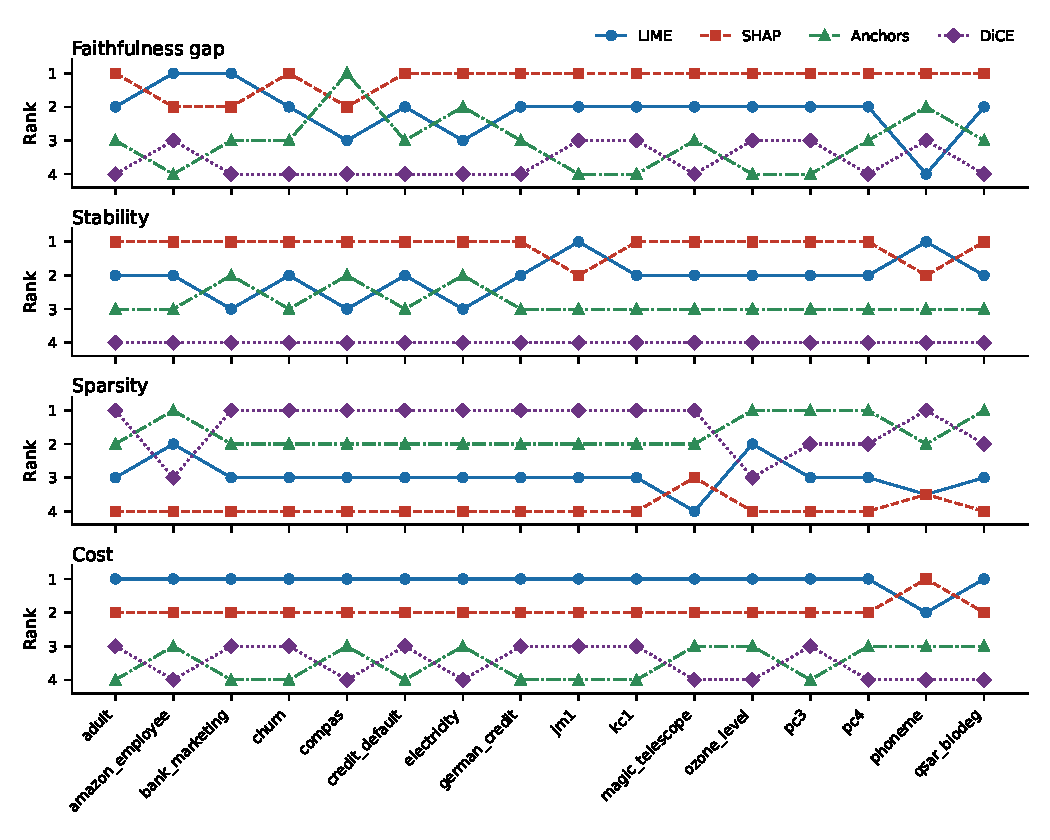
\includegraphics[width=\textwidth]{figures/fig1.pdf}
\caption{Rank of each method (1 = best) on each dataset, one panel per measure. Adult is
the first dataset; the others are in alphabetical order.}
\label{fig:ranks}
\end{figure*}

Table~\ref{tab:primary} gives the mean rank of each method and the agreement of the
rankings between datasets, and Figure~\ref{fig:ranks} shows the rank of each method on
each dataset. The decision rule gives the following. For the faithfulness gap
($\bar{\rho}=$~0.67), the order of the methods is shared between datasets, with a strength that is not determined: the interval contains 0.5. For
stability ($\bar{\rho}=$~0.88),
the order of the methods generalises: it is shared between datasets and the interval lies above 0.5. For sparsity
($\bar{\rho}=$~0.79), the order of the methods generalises: it is shared between datasets and the interval lies above 0.5.
For cost ($\bar{\rho}=$~0.87),
the order of the methods generalises: it is shared between datasets and the interval lies above 0.5.

The agreement between seeds inside a dataset is 0.948,
0.973, 0.995 and
0.975 for the four measures in the same order. On the
instances that all four methods explained, the agreement between datasets is
0.67, 0.85,
0.84 and 0.87.
The number of measures for which the decision differs from the one above is
zero. In a check made after the results were seen, the analysis was
repeated with one software-defect dataset in place of the four (13
datasets), once for each of the four. The agreement between datasets was
then 0.64 to 0.67, 0.85 to
0.88, 0.76 to 0.77
and 0.86 to 0.87, and the decision of the
rule was the one above in 16 of the 16 cases.

Computed for each classifier alone, the agreement between datasets is, in the order
faithfulness gap, stability, sparsity and cost: 0.73,
0.80, 0.87 and
0.85 for logistic regression;
0.71, 0.80,
0.71 and 0.79 for the
random forest; 0.64, 0.82,
0.78 and 0.89 for
XGBoost; and 0.64, 0.82,
0.88 and 0.91 for the
multilayer perceptron.

\begin{table}[t]
\centering
\caption{Number of the 15 other datasets in which a pair of methods is in the same order as on Adult, by measure.}
\label{tab:adult}
\small
\begin{tabular}{@{}lrrrr@{}}
\toprule
Pair & Faith. & Stab. & Spars. & Cost \\
\midrule
LIME--SHAP & 13 & 13 & 13 & 14 \\
LIME--Anchors & 12 & 12 & 15 & 15 \\
LIME--DiCE & 14 & 15 & 13 & 15 \\
SHAP--Anchors & 14 & 15 & 15 & 15 \\
SHAP--DiCE & 15 & 15 & 15 & 15 \\
Anchors--DiCE & 10 & 15 & 10 & 7 \\
\bottomrule
\end{tabular}
\end{table}


Table~\ref{tab:adult} counts, for each pair of methods, the datasets in which the pair is
in the same order as on Adult. Of the 24 comparisons,
12 hold on all 15 other datasets and
21 on at least 12; the three that hold on fewer all
concern Anchors and DiCE, whose order on cost is that of Adult on
7 datasets (exact 95\% interval
0.21 to 0.73).
Between two
datasets the rank of a method changes by up to 3,
2, 2 and 1
positions on the four measures, and 3, 2,
2 and 2 of the four methods are ranked first
on at least one dataset.

Three counts made after the results were seen describe how the measures behave. An
explanation names on average 9.5 features for LIME,
21.3 for SHAP, 3.0 for
Anchors and 3.0 for DiCE, and the faithfulness gap masks
6.5, 8.0,
2.1 and 2.7 of
them. With the median of a run in place of its mean, DiCE is faster than Anchors on
14 of the 16 datasets, against
8 with the mean: a small share of very slow searches
decides the planned order of the two.

Of the variance of the 1,280 run means, the method accounts for
19\%, 65\%,
43\% and 6\% (faithfulness
gap, stability, sparsity, cost), the dataset for 40\%,
14\%, 25\% and
8\%, and the interaction of method and dataset for
9\%, 9\%,
10\% and 17\%. The
permutation $p$ of the interaction is $<$0.001,
$<$0.001, $<$0.001 and
$<$0.001. For cost these are shares of raw times, in which a
few slow conditions dominate: the interaction of method, dataset and classifier holds
43\%.

\section{Result discussion and conclusions}

The hypothesis is supported on each of the four measures: the order of the methods agrees
between datasets more than chance. For stability, sparsity and cost the interval of the
agreement lies above 0.5, so by the rule fixed in advance the order generalises. For the
faithfulness gap the interval runs from 0.49 to
0.85; its lower end falls just below 0.5, and the rule gives a shared
order of undetermined strength. We report that outcome as the rule gives it. That the
orders are not unrelated was to be expected; the evidence of the study is the size of the
agreement and the identity of the pairs that change.

The agreement between datasets, from 0.67 to
0.88, is below the agreement between seeds on every
measure, which runs from 0.948 to
0.995. Changing the dataset therefore
alters the order more than repeating the study on the same dataset does, and since the
agreement between seeds is a conservative reference, the difference is not produced by
the comparison. The interaction of method and dataset is significant on every measure.

Much of the agreement on sparsity, stability and cost follows from the output format, the
algorithm and the settings of the methods, and would be expected on any dataset. LIME is set
to 10 features and the kernel variant of SHAP returns at most 10, while the tree variant
weights every feature, so SHAP cannot be the sparser of the two where a dataset has more
than 10 encoded features. DiCE searches at random and each stability copy is explained
with new draws, which places it last on stability on every dataset and favours the
deterministic tree variant of SHAP. LIME and SHAP are faster than the two search methods
on every dataset. The orders that the data decide are fewer: that of Anchors and DiCE on
sparsity and on cost, and that of LIME, SHAP and Anchors on the faithfulness gap. There
the first place changes little, SHAP having the largest gap on
13 of the 16 datasets, while LIME and
Anchors each range from rank 1 to rank
4. The order of Anchors and DiCE is that of Adult on
7 to 10 of
the 15 other datasets on three measures (Table~\ref{tab:adult}), and
on cost it turns on the slow searches of DiCE. For images, metric results on one dataset
did not necessarily hold on others~\cite{gevaert2024evaluating}; for these four methods
on tabular data they mostly do, in part for the reasons just given.

No method is first on all measures, and the order on sparsity is close to the reverse of
the order on the faithfulness gap (Table~\ref{tab:primary}). That opposition is in part
built into the two definitions: the gap masks only the features an explanation names, so
a method that names fewer features has fewer of them masked, as the counts above show. A
gap measured at an equal number of masked features would separate the two; it needs the
fitted classifiers and is left for further work. The size of a measure
is another matter: the dataset accounts for more of the variance of the faithfulness gap
than the method does, so a value of the gap cannot be carried from one dataset to another
even where the order can.

\textit{Possible sources of error.} Explanations are computed on encoded features, so a
categorical variable counts as several features. Anchors and DiCE are compared with LIME
and SHAP through the features they name, not through their native output, so the
faithfulness gap and the stability measure depend on how many features a method names.
Each method has one configuration, and the orders described above as following from it
could differ with another. DiCE treats one-hot columns as continuous, so a counterfactual
can hold a value that no category has. The failures are concentrated in three conditions of DiCE; the analysis of the
instances that all four methods explained gives the same decisions. Four of the datasets
are software-defect data of one family, so the sixteen are less
independent than their number suggests; with the family counted once, in the check
reported above, the decisions do not change. With four methods a ranking
takes few values, and the value 0.5 of the rule is a convention. The datasets are binary
classification tasks from one repository; nine of the
sixteen have only numeric features and one
only categorical ones. Cost is wall time on one machine. Two analyses depart from the
plan, as its log records: the variance shares are a balanced decomposition of sums of
squares and not the mixed model named there, and cost relative to the prediction time
was not computed. The aligned-rank check of the interaction, the matrix of dataset pairs,
the frontier of cost and faithfulness, the secondary measures and the failure rate of
every condition were computed as planned and are in the archive, not in this paper; the
aligned-rank check confirms the test of the interaction and gives no comparable shares.

The conclusions are:
\begin{enumerate}
\setlength{\itemsep}{0pt}
\item The order of LIME, SHAP, Anchors and DiCE, as configured here, agrees across
16 tabular datasets on the four measures, on the faithfulness gap
with a strength that this study does not determine. On sparsity, stability and cost much
of that agreement follows from the output format, the algorithm and the settings of the
methods, and is not evidence about datasets.
\item Where the data decide the order, the first place changes little: SHAP has the
largest faithfulness gap on 13 of the
16 datasets. The order of Anchors and DiCE is the one that changes,
and should not be taken from a single dataset.
\item The order on one measure does not transfer to another, and the opposition between
sparsity and the faithfulness gap is partly a consequence of their definitions. It should
not be read as a property of the methods until faithfulness is measured independently of
the number of features an explanation names.
\end{enumerate}
Further research should measure the faithfulness gap at an equal number of masked
features, test whether the result holds for multiclass and regression tasks, for datasets
from other repositories and with configurations tuned for each dataset, and examine which
properties of a dataset go with a change of order, a question this design does not
answer.

\section*{Data and code availability}
\iffull
The datasets are public (OpenML). The plan, the code, the per-instance results and the
generators of every table and figure are at
\url{https://github.com/jonnabio/xai-eval-framework}, archived at \paperfarchive.
\else
The datasets are public. The plan, the code, the per-instance results and the generators
of every table and figure are in a public archive whose address is omitted for
double-blind review.
\fi

%% The journal requires this declaration, with the name of the tool and the reason for
%% its use. Text approved by the author on 2026-10-05 and confirmed for submission on
%% 2026-10-12; it is not changed without the author's approval.
\section*{Declaration on the use of generative AI}
The author used the AI tool Claude (Anthropic), under the author's direction, to help
write the analysis code, edit the English text and format the references. The research
question, the plan, the design and the interpretation are the author's. The author
reviewed all content and takes full responsibility for it.

%% Author's rule (2026-10-05) and the journal's template: every reference prints its DOI
%% as an active URL. The style writes \href{https://doi.org/...}{doi:...}; print the URL.
{\renewcommand{\href}[2]{\url{#1}}
\bibliographystyle{elsarticle-num}
\bibliography{references}}

\end{document}
